% ==============================================================================
% 第二章: 布尔代数与卡诺图 - 实战演算
% ==============================================================================
\section{布尔代数与K-Map}

\subsection{布尔代数速查}

\begin{formula}[核心定律]
\begin{tabular}{ll}
\textbf{幂等律:} & $A + A = A$, $A \cdot A = A$ \\
\textbf{补余律:} & $A + \bar{A} = 1$, $A \cdot \bar{A} = 0$ \\
\textbf{吸收律:} & $A + AB = A$, $A(A+B) = A$ \\
\textbf{德摩根:} & $\overline{A+B} = \bar{A}\bar{B}$, $\overline{AB} = \bar{A}+\bar{B}$ \\
\textbf{异或:} & $A \oplus B = A\bar{B} + \bar{A}B$ \\
\end{tabular}
\end{formula}

\subsection{卡诺图 - 4变量标准模板}

\begin{algorithm}[K-Map绘制步骤]
\begin{enumerate}
\item 确定变量排列: 行 = $AB$, 列 = $CD$ (格雷码!)
\item 标注格雷码顺序: 00, 01, 11, 10
\item 填入真值表中的1
\item 圈相邻的1 (大小必须是2的幂)
\item 写出最简SOP
\end{enumerate}
\end{algorithm}

\begin{center}
\textbf{4变量K-Map模板 (格雷码标注)}
\vspace{3pt}

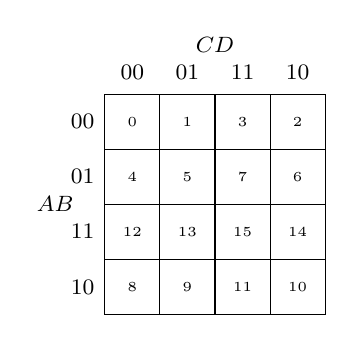
\begin{tikzpicture}[scale=0.7]
% 画格子
\draw (0,0) grid (4,4);
% 标注CD (列)
\node at (0.5, 4.4) {\footnotesize 00};
\node at (1.5, 4.4) {\footnotesize 01};
\node at (2.5, 4.4) {\footnotesize 11};
\node at (3.5, 4.4) {\footnotesize 10};
\node at (2, 4.9) {\footnotesize $CD$};
% 标注AB (行)
\node at (-0.4, 3.5) {\footnotesize 00};
\node at (-0.4, 2.5) {\footnotesize 01};
\node at (-0.4, 1.5) {\footnotesize 11};
\node at (-0.4, 0.5) {\footnotesize 10};
\node at (-0.9, 2) {\footnotesize $AB$};
% 填入变量索引
\node at (0.5,3.5) {\tiny 0};
\node at (1.5,3.5) {\tiny 1};
\node at (2.5,3.5) {\tiny 3};
\node at (3.5,3.5) {\tiny 2};
\node at (0.5,2.5) {\tiny 4};
\node at (1.5,2.5) {\tiny 5};
\node at (2.5,2.5) {\tiny 7};
\node at (3.5,2.5) {\tiny 6};
\node at (0.5,1.5) {\tiny 12};
\node at (1.5,1.5) {\tiny 13};
\node at (2.5,1.5) {\tiny 15};
\node at (3.5,1.5) {\tiny 14};
\node at (0.5,0.5) {\tiny 8};
\node at (1.5,0.5) {\tiny 9};
\node at (2.5,0.5) {\tiny 11};
\node at (3.5,0.5) {\tiny 10};
\end{tikzpicture}
\end{center}

\subsection{K-Map圈法规则}

\begin{pitfall}[K-Map圈法陷阱]
\begin{itemize}
\item 圈必须是 $2^n$ 个1: 1, 2, 4, 8, 16...
\item 圈可以跨边界(环绕)!
\item 四角可以组成一个圈!
\item 圈越大越好 (消去更多变量)
\item 每个1至少被圈一次
\item 不要重复圈 (除非必要)
\end{itemize}
\end{pitfall}

\begin{example}[K-Map实战例题]
\textbf{化简:} $F(A,B,C,D) = \sum m(0,1,2,5,7,8,9,10,14)$

\textbf{Step 1: 填入K-Map}

\begin{center}
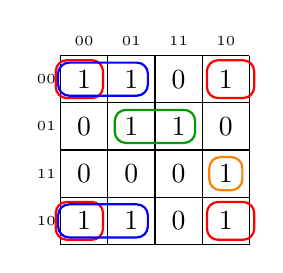
\begin{tikzpicture}[scale=0.6]
\draw (0,0) grid (4,4);
% 列标签
\node at (0.5, 4.3) {\tiny 00};
\node at (1.5, 4.3) {\tiny 01};
\node at (2.5, 4.3) {\tiny 11};
\node at (3.5, 4.3) {\tiny 10};
% 行标签
\node at (-0.3, 3.5) {\tiny 00};
\node at (-0.3, 2.5) {\tiny 01};
\node at (-0.3, 1.5) {\tiny 11};
\node at (-0.3, 0.5) {\tiny 10};
% 填入值
\node at (0.5,3.5) {1}; % m0
\node at (1.5,3.5) {1}; % m1
\node at (2.5,3.5) {0}; % m3
\node at (3.5,3.5) {1}; % m2
\node at (0.5,2.5) {0}; % m4
\node at (1.5,2.5) {1}; % m5
\node at (2.5,2.5) {1}; % m7
\node at (3.5,2.5) {0}; % m6
\node at (0.5,1.5) {0}; % m12
\node at (1.5,1.5) {0}; % m13
\node at (2.5,1.5) {0}; % m15
\node at (3.5,1.5) {1}; % m14
\node at (0.5,0.5) {1}; % m8
\node at (1.5,0.5) {1}; % m9
\node at (2.5,0.5) {0}; % m11
\node at (3.5,0.5) {1}; % m10
% 圈1: 四角 (0,2,8,10) - 红色
\draw[red, thick, rounded corners] (-0.1,3.9) rectangle (0.9,3.1);
\draw[red, thick, rounded corners] (3.1,3.9) rectangle (4.1,3.1);
\draw[red, thick, rounded corners] (-0.1,0.9) rectangle (0.9,0.1);
\draw[red, thick, rounded corners] (3.1,0.9) rectangle (4.1,0.1);
% 圈2: (0,1,8,9) - 蓝色
\draw[blue, thick, rounded corners] (-0.05,3.85) rectangle (1.85,3.15);
\draw[blue, thick, rounded corners] (-0.05,0.85) rectangle (1.85,0.15);
% 圈3: (5,7) - 绿色
\draw[green!60!black, thick, rounded corners] (1.15,2.85) rectangle (2.85,2.15);
% 圈4: (14) - 单独
\draw[orange, thick, rounded corners] (3.15,1.85) rectangle (3.85,1.15);
\end{tikzpicture}
\end{center}

\textbf{Step 2: 识别圈}
\begin{itemize}
\item \textcolor{red}{圈1 (四角):} m(0,2,8,10) $\to$ $\bar{B}\bar{D}$
\item \textcolor{blue}{圈2 (跨边):} m(0,1,8,9) $\to$ $\bar{B}\bar{C}$
\item \textcolor{green!60!black}{圈3:} m(5,7) $\to$ $\bar{A}BD$
\item \textcolor{orange}{圈4:} m(14) $\to$ $AB\bar{C}D$
\end{itemize}

\textbf{Step 3: 写出最简式}
\[
F = \bar{B}\bar{D} + \bar{B}\bar{C} + \bar{A}BD + AB\bar{C}D
\]
\end{example}

\subsection{POS形式化简}

\begin{algorithm}[POS化简步骤]
\begin{enumerate}
\item 在K-Map中圈0 (不是圈1!)
\item 对每个圈写出maxterm
\item maxterm是变量的OR
\item 结果是所有maxterm的AND
\end{enumerate}

\textbf{技巧:} 圈0时,变量取值与SOP相反:
\begin{itemize}
\item 变量=0 $\to$ 写变量本身
\item 变量=1 $\to$ 写变量的补
\end{itemize}
\end{algorithm}

\subsection{Don't Care条件}

\begin{keybox}[Don't Care (X) 使用]
\begin{itemize}
\item Don't Care可以当1用来扩大圈
\item Don't Care也可以当0用来忽略
\item 目标: 让圈尽可能大
\item 最终表达式中不包含X
\end{itemize}
\end{keybox}
